\documentclass[uplatex,dvipdfmx]{jsarticle}

\usepackage[uplatex,deluxe]{otf} % UTF
\usepackage[noalphabet]{pxchfon} % must be after otf package
\usepackage{stix2} %欧文&数式フォント
\usepackage[fleqn,tbtags]{mathtools} % 数式関連 (w/ amsmath)
\usepackage{hira-stix} % ヒラギノフォント&STIX2 フォント代替定義(Warning回避)
\usepackage{amsmath}
\usepackage{url}

\setcounter{tocdepth}{3}
\usepackage{float}
\usepackage{moreverb}
\usepackage{lscape}
%\pagestyle{empty}
%\usepackage{wrapfig}
%\usepackage{url}
%\usepackage{EasyLayout}

\usepackage{ascmac}
\usepackage{xurl}

\begin{document}

\title{危険交差点警告システム}
\author{25G1051 近藤巧望}
%\date{6月12日(木)}
\maketitle
\section{はじめに}
%はじめにのセクションでは,研究の背景や目的を簡潔に記述する.

\subsection{社会的背景}
\indent
自転車は温室効果ガスを排出しない移動手段であり,環境に優しい交通手段として注目されている.
また,日本の自転車保有台数は約6870万台つまり約二人に1台となっており,自転車は現在でも使う人が多い他,
交通渋滞の緩和や健康促進,地球温暖化等の環境問題への配慮の観点から,政府からも自転車活用推進法に基づき,自転車の利用が推奨されている.
\cite{ref:koutuusyou_1}
\cite{ref:koutuusyou_2}
\par
しかし交通事故に焦点を当てると,自転車関連事故件数及び自転車乗用中死者・重傷者数は減少傾向にある一方で,全交通事故に占める構成比は近年増加傾向にある.
\cite{ref:sonpo_1}
\par

\subsection{問題点}
\indent
自転車での出会い頭衝突の事故の多さが問題である.
全自転車事故中で出会い頭衝突による事故は、自転車事故全体のおよそ5割を占めている.
また,自転車事故は,特に十字路やT字路で発生することが多く,これらの場所では視界が遮られたり,信号の認識が難しかったりするため,事故が起こりやすい.
さらに,自転車事故の多くは法令違反や不注意によるものであり,標識や信号を無視したり,携帯電話を使用したりすることなどが原因として挙げられる.
\cite{ref:keisatu_1}
\par
しかし実際のところ,法令違反や不注意を完全に無くすことは難しい.
それに加え,法規制や啓発活動だけでは、すべての利用者の行動変容を促すのは難しいとされており,事故の根本的な解決には至らない.
そのため,出会い頭衝突の事故を減らすためには,使用者に自動かつ適切な注意喚起を行う仕組みが必要である.
\par
そこでわたしたちは,出会い頭衝突の事故を減少させるために,交差点などの危険な場所での注意喚起システムを提案する.
\par
%一般的な社会的背景を記述したパラグラフを複数配置, パラグラフの終わりは\parを入れる。
%最終パラグラフにはアイデアを記述する.



\subsection{目的}

\indent
本提案の目的は,自転車同士での出会い頭衝突を防ぐための対策を考え,自転車事故の発生を減少させることであり,
自転車事故の発生が減少することで,事故による負傷者や死者数を減少させることができると考えられる.
\par

\subsection{主張}
自転車搭乗者の注意力の限界を補い事故を防げる方法として,AIによる画像認識技術を用いた警告装置を考えた.
特に,自転車事故の発生が多い交差点やT字路を認識し,搭乗者に警告を行うことで,事故を未然に防ぐことができると考える.
ここでは,GPSと連携し,自転車の位置情報を取得することで,危険な交差点やT字路を事前に特定し,搭乗者に警告を行う仕組みを提案する.
また本稿では,交差点での動作に限定させて考える.



\section{解決策としての提案手法}
%アイデアを実現する概要図を入れてその内容を説明する.
\subsection{提案手法の概要}
\begin{center}
  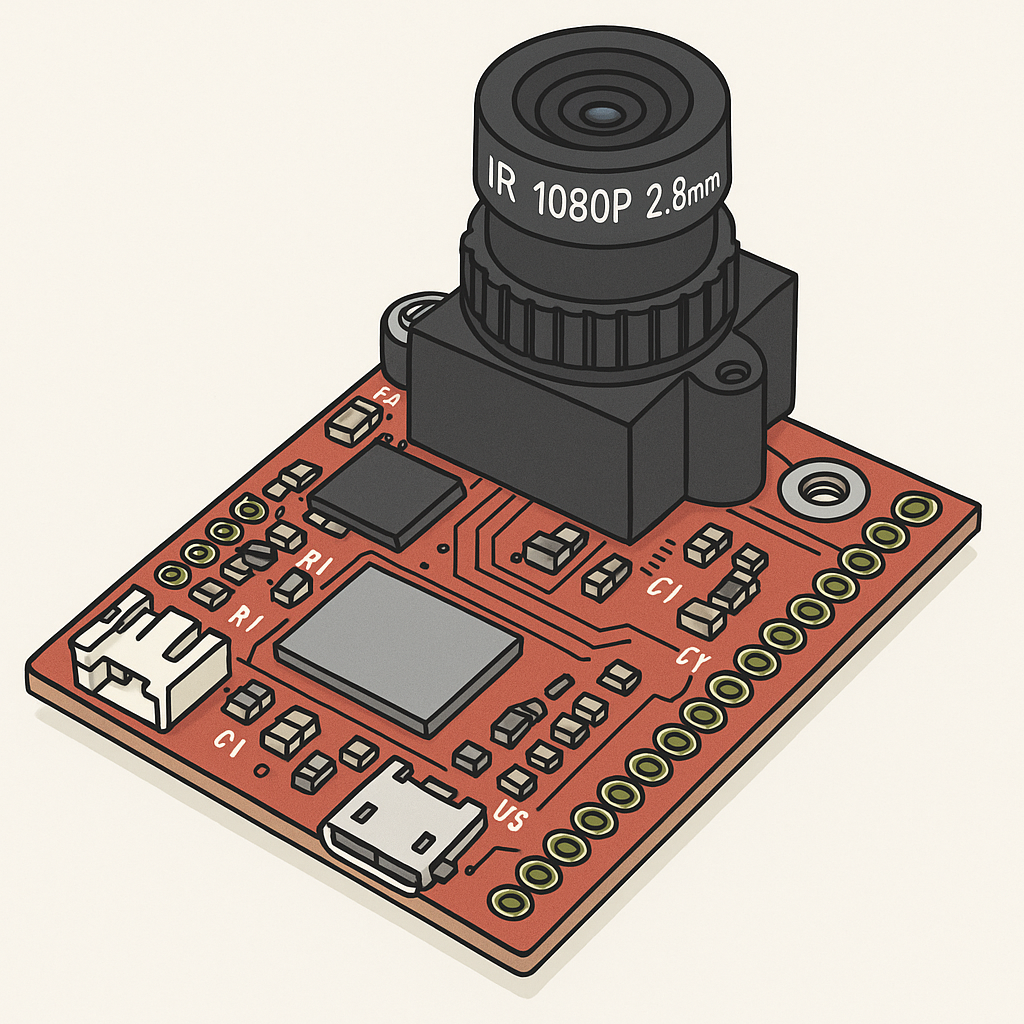
\includegraphics[width=8cm]{./Figs/OpenMV_image.png}
  
  \vspace{2mm}
  画像1 OpenMV Cam H7 Plus モジュール.小型で低消費電力のマイクロコントローラボードであり,AI による画像認識が可能.\cite{ref:openmv}
\end{center}

\indent
装置の概要としては,カメラ付きの小型コンピュータ「OpenMV Cam」を自転車のハンドル部分に取り付け,周囲の状況をリアルタイムで監視する.
OpenMV Camには「OV5640イメージセンサー」というカメラ部品が搭載されており,これを使って交差点を撮影する.
撮影した画像は,AIによる画像認識技術で解析し,交差点やT字路を自動的に検出する.
具体的には、カメラ画像から白線、標識、交差点の形状などの道路の特徴を抽出し、機械学習モデルによって交差点やT字路を判別する。
判別には、エッジ検出やパターンマッチングなどの画像処理手法を組み合わせる。
もし交差点が検出された場合は,搭乗者に音声や振動などで警告を行い,注意を促す仕組みである.
\par
ここからは,主に十字路での事故を想定したものとして考える.
装置に必要な部品を表1に,装置の概念図を図1に示す.

\begin{table}[h]
  \centering
  \caption{装置に必要な部品.}
  \label{tab:parts}
  \begin{tabular}{|c|l|l|}
    \hline
    項目 & 使用部品 & 備考\\ \hline
    1 & OpenMV Cam H7 Plus(基盤+カメラ) & 焦点距離:2.8mm最大解像度:2592x1944(5MP)画素数:640\\ \hline
    2 & モバイルバッテリー & 電力:5000mAh \\ \hline
    3 & 圧電アクティブブザー & 音量:85dB前後 \\ \hline
    4 & 防水ケース・固定具 & 防水プロジェクトボックス、ベルクロ等含む \\ \hline
    5 & 配線・スイッチ & スイッチはon/offを切り替えるのに使用 \\ \hline
  \end{tabular}
\end{table}

\begin{figure}[H]
  \centering
  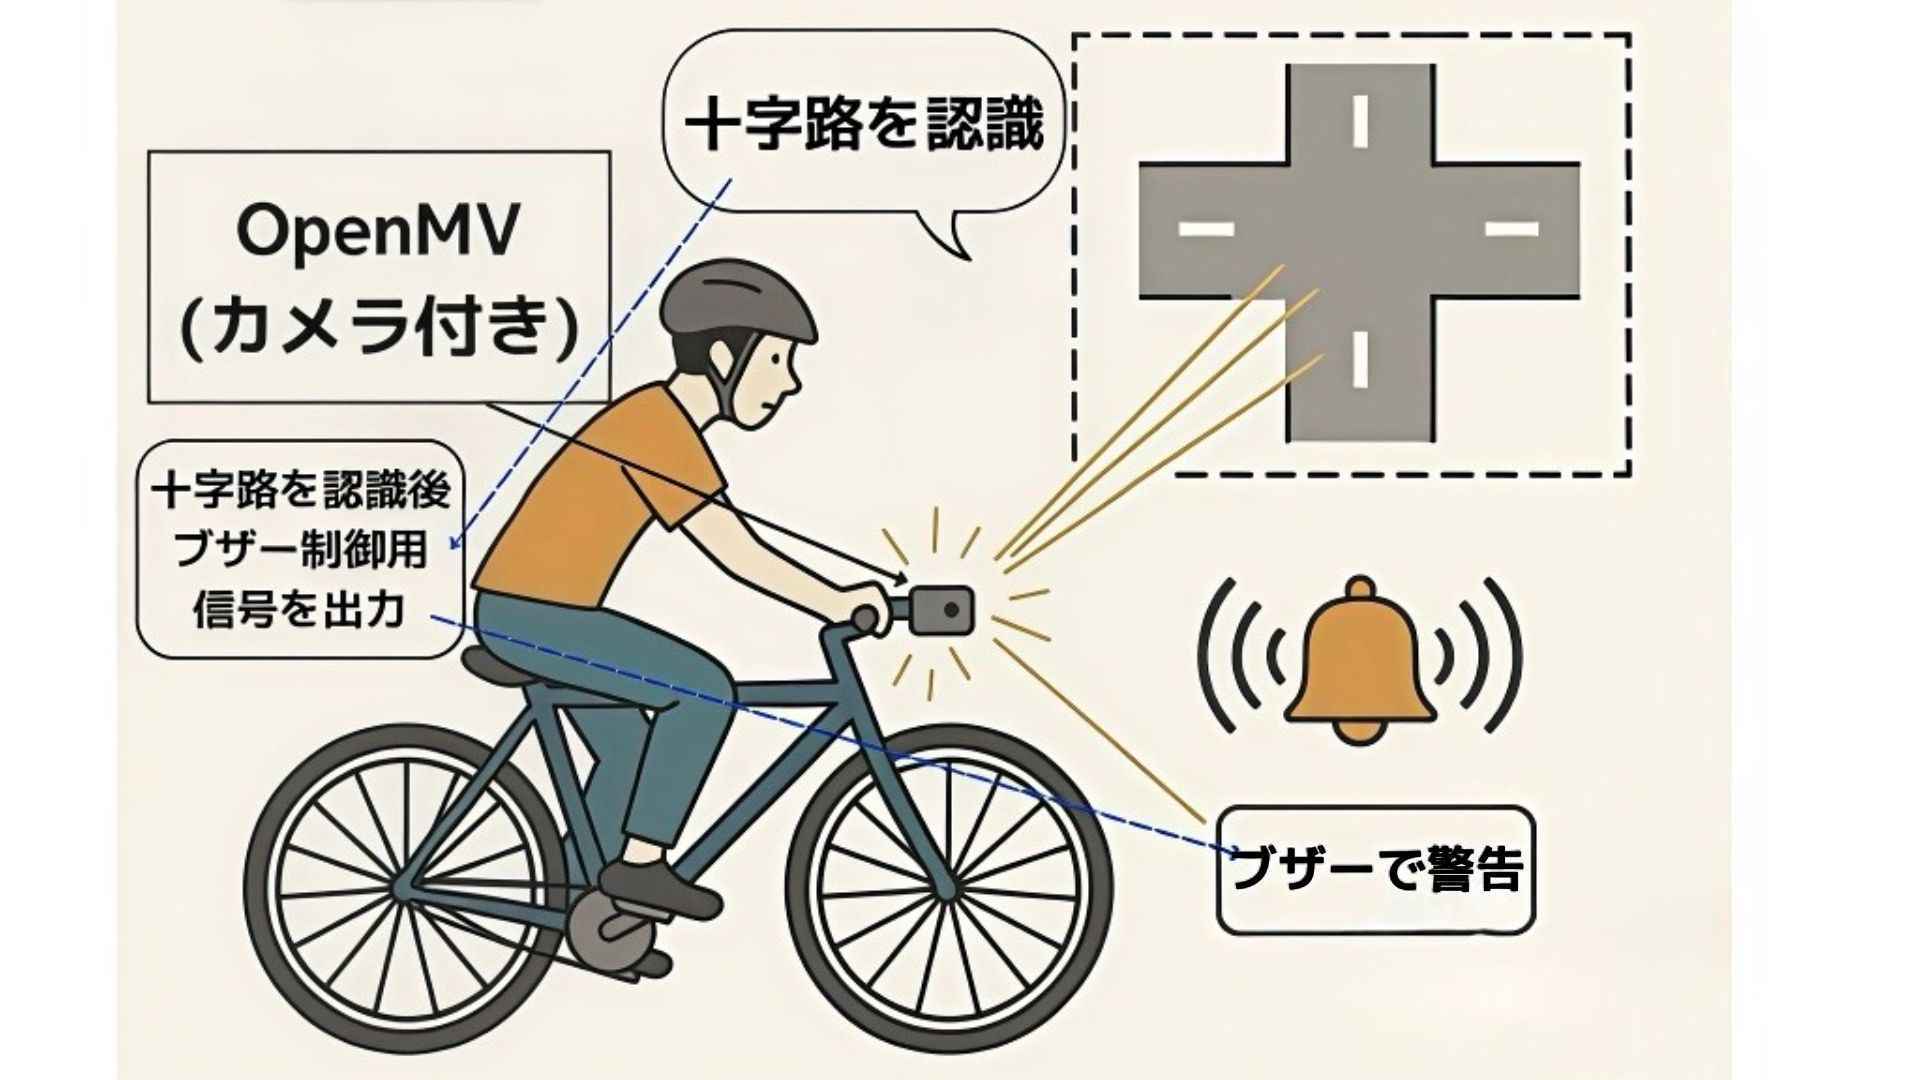
\includegraphics[width=14cm]{./Figs/gainenzu.jpg}
  \caption{十字路認識システムの概念図.OpenMV Cam H7 Plusで十字路を認識し,ブザー音で搭乗者に警告を行う.ハンドル中央部または自転車のカゴ前部に取り付ける.}
  \label{fig:idea}
\end{figure}

\par
%装置の構成要素を表1に示す.

\subsection{提案手法の装置構成}
\indent
表1に示すように,本装置は主に4つの部品から構成される.
図1のように,中心となるのはOpenMV Cam H7 Plusであり,入力と処理を担当する.
OpenMV Camは小型ながら高性能なマイクロコントローラとOV5640イメージセンサー(最大2592×1944ピクセル)を搭載している.
このセンサーにより,遠くの交差点や標識も高解像度で撮影できる.
また,OpenMV CamはPythonベースでプログラム可能であり,
ユーザーが独自の画像認識アルゴリズムを柔軟に実装できる.
また,類似したものにOpenCVというソフトウェアがあるが,
一般的なPCやRaspberry PiなどでOpenCVを用いるシステムと比べて,
OpenMV Camは小型・低消費電力であるため,自転車への搭載に適している.
\cite{ref:opencv}
\par
モバイルバッテリーは,OpenMV Cam H7 Plusやブザーなど装置全体に電力を供給する役割を担う.
モバイルバッテリーは5000mAhの容量を持ち,長時間の使用が可能であり,これもOpenMV Cam H7 Plusと同様に自転車のハンドル部分に取り付けることができる.
また,モバイルバッテリーはUSB接続で簡単に充電できるため,日常的なメンテナンスも容易である.
\par
圧電アクティブブザーは,搭乗者に警告を伝えるための音声出力装置であり,
風切り音などの騒音環境下でも確実に注意喚起できるよう,圧電スピーカーではなく圧電アクティブブザーを採用している.
音量はプログラムで調整可能であり,今後,実際の検証に応じて,
騒音問題とならず,かつ搭乗者に確実に届く音量に設定できる.
\par
ケース・固定具は,OpenMV Cam H7 Plusやモバイルバッテリーを
自転車のハンドル部分などに安全かつ確実に取り付けるために使用する.
防水については,OpenMV本体を防水プロジェクトボックス内に密閉収納し、レンズ部には防滴処理を施す.
ブザーは防水性のあるものを選定し,モバイルバッテリーも防水ケースに収納することで,雨天時でも使用可能とする.
使用時以外はスイッチをオフにすることで,装置の電力消費を抑えることができる.
\par

\subsection{提案手法のシステム構成}

\begin{figure}[h]
  \centering
  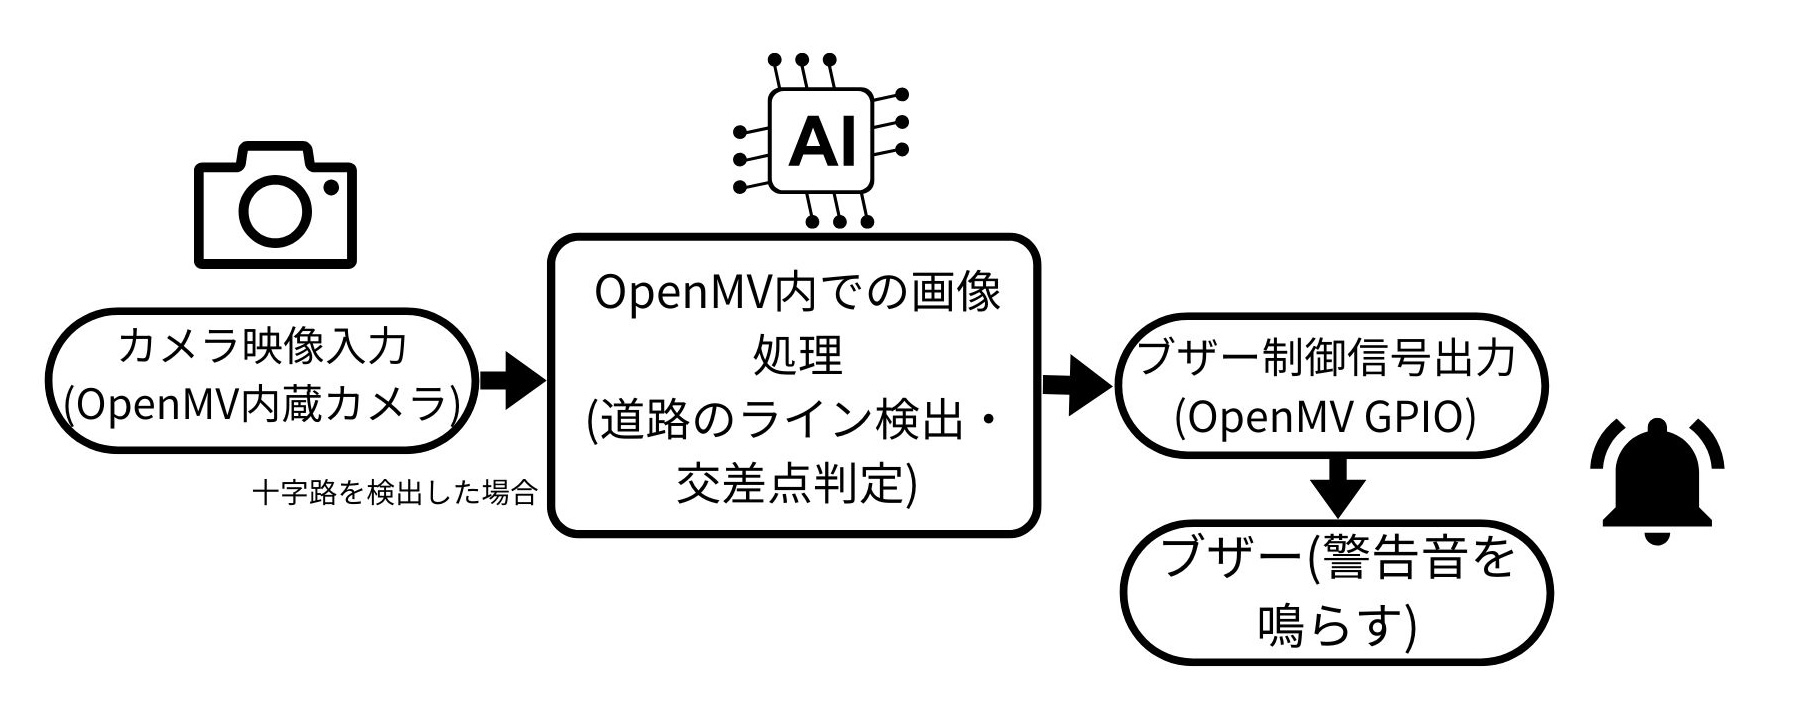
\includegraphics[width=14cm]{./Figs/system.jpg}
  \caption{十字路認識システムのシステム構成図.入力と処理をOpenMV Cam H7 Plusが担当し,出力を圧電アクティブブザーが行う.}
  \label{fig:system}
\end{figure}

ここでは,システムの詳細な構成と動作フローについて説明する.図2に提案手法のシステム構成図を示す.
本システムは,OpenMV Cam H7 Plusを中心に,周囲の状況を監視するカメラ,警告用の圧電アクティブブザー,
電源供給用のモバイルバッテリーで構成されている.ブザーはOpenMV Cam H7 PlusのGPIOピンによって制御される.
図2が示すように,システムの主な機能は,カメラ画像から交差点を自動的に検出し,搭乗者にリアルタイムで警告を行うことである.
入力はカメラから取得される画像データ,出力は圧電アクティブブザーによる音声信号となる.
動作の流れとしては,カメラが前方の映像を常時撮影し,OpenMV Cam H7 Plusがその画像をAI画像認識アルゴリズムで解析する.
交差点が検出された場合,GPIOピンを通じてブザーが作動し,搭乗者に危険を知らせる.
さらに,誤検出を防ぐため,複数フレームでの連続判定や,環境光の変化に応じたしきい値調整などの工夫も必要である.
\par
AI画像認識アルゴリズムは,まず入力画像から道路の白線や標識,交差点の形状などの特徴を抽出し,
これらの特徴量をもとに交差点の有無を判定する仕組みである.
具体的には,画像の中で線や輪郭などの変化が大きい部分(エッジ)を見つける「エッジ検出」や,
物体の外枠を取り出す「輪郭抽出」といった画像処理手法を用いる.
さらに,明るさの違いによる影響を減らすために,画像の明るさを調整したり,ノイズを除去したりする「前処理」も行う.
これらの処理で得られた情報をもとに,機械学習モデルによって交差点のパターンを認識する.
また,照度変化やノイズに対しても安定した認識ができるよう,画像の明るさに応じて自動的にしきい値を調整する工夫も取り入れる.
\par

\vspace{3cm}

\section{提案手法の実現可能性の評価と妥当性の検証}

\subsection{主張・手法のまとめ}
\indent
本提案は,自転車搭乗者の注意力の限界を補い,出会い頭衝突の事故を防ぐための十字路認識システムである.
具体的には,OpenMV Cam H7 Plusを用いて十字路を認識し,搭乗者に警告を行う仕組みである.
このシステムは,小型・低消費電力であり,自転車への搭載が容易であるため,日常的な使用にも適している.
また,AIによる画像認識技術を用いることで,従来の法令違反や不注意による事故防止策と比べて,より効果的な注意喚起が可能であると考えられる.
\par

%提案手法の実現可能性を評価する.
\subsection{実現可能性の評価}
\indent
まず,提案手法の実現可能性について評価する.
OpenMV Cam H7 Plusで十字路を認識する際,認識可能な距離はOpenMV Cam H7 Plusのカメラの焦点距離に依存する.
表1の通り,OpenMV Cam H7 Plusのカメラは焦点距離が2.8mmであり,最大解像度は2592x1944ピクセルである.
これらを下に,十字路を認識するための距離を計算する.
センサー横幅を計算すると,約3.63mmとなるが、実際のOV5640センサーは1/4インチ型であり、
仕様上の実測横幅は約4.8mmであるため、ここでは約4.8mmを用いる。
認識できる距離については,OpenMV H7 Plusのカメラの性能や周囲の天候・時間帯に依存するが,OpenMV H7 Plusの標準レンズを使用した場合,
十字路の交差部分の幅を5m(5000mm)とし,十字路の交差部が画像で少なくとも100ピクセル横幅で写ると仮定すると,
この装置が認識できる距離は,

\[
D_{\text{max}} = \frac{W_t × f × P_{\text{img}}}{P_{\text{min}} × W_{\text{sen}}}
\]
\hspace{1cm}($D_{\text{max}}$:最大認識距離, $W_t$:十字路の交差部の幅, $W_{sen}$:センサーの横幅, $f$:焦点距離, $P_{\text{img}}$:撮影解像度の横ピクセル数
, $P_{\text{min}}$:最小認識ピクセル数)

\vspace{1cm}

を用いて求められる.\cite{ref:kyori}
よって,


\[
D_{max} = \frac{5000 \times 2.8 \times 640}{100 \times 4.8} = \frac{8{,}960{,}000}{483} \approx 18{,}667\,\mathrm{mm} = {18.7\,\mathrm{m}}
\]

\vspace{1cm}
と計算できる.
したがって,OpenMV Cam H7 Plusを用いた場合,十字路を約18.7mの距離から認識できることがわかる.
\par
しかし,実際の使用環境では,周囲の天候や時間帯によって認識精度が変化する可能性がある.
例えば,夜間や雨天時には視界が悪くなるため,認識精度が低下する可能性がある.
また,周囲の障害物や交通量によっても認識精度が影響を受ける可能性がある.
そのため,実際の使用環境においては,18.7mの距離からの認識が保証されるわけではない.
GPSとの連携や,アプリケーションとしての導入を検討することで,より正確な位置情報を取得し,
認識精度を向上させることが可能であると思われる.
\par
\begin{table}[h]
  \centering
  \caption{装置に使用する部品の重量}
  \label{tab:parts}
  \begin{tabular}{|c|l|l|}
    \hline
    項目 & 使用部品 & 重量\\ \hline
    1 & OpenMV Cam H7 Plus(基盤+カメラ) & 約50g\\ \hline
    2 & モバイルバッテリー & 約150g\\ \hline
    3 & 圧電アクティブブザー & 約20g\\ \hline
    4 & 防水ケース・固定具 & 約100g\\ \hline
    5 & 配線・スイッチ & 約30g\\ \hline
  \end{tabular}
\end{table}

\subsection{妥当性の検証}
\indent
次に,提案手法の妥当性についてを説明する.
提案手法は,OpenMV Cam H7 Plusを用いて十字路を認識し,搭乗者に警告を行うものである.
十字路を認識するためには,OpenMV Cam H7 Plusのカメラが十分な解像度と焦点距離を持っている必要がある.
OpenMV Cam H7 Plusのカメラは最大解像度が2592x1944ピクセルであり,焦点距離が2.8mmである.
これらの性能は,十字路を認識するために十分であると考えられる.
また,OpenMV Cam H7 PlusはPythonベースでプログラム可能であり,
ユーザーが独自の画像認識アルゴリズムを柔軟に実装できるため,十字路認識の精度を向上させることが可能である.
さらに,提案手法は小型・低消費電力であるため,自転車への搭載が容易であり,日常的な使用にも適している.
表2に示すように,装置全体の重量は軽量であり,自転車への取り付けや取り外しが簡単である.
また,提案手法は,AIによる画像認識技術を用いているため,従来の法令違反や不注意による事故防止策と比べて,
より効果的な注意喚起が可能であると考えられる.
さらに,提案手法は自転車搭乗者の注意力の限界を補い,事故を防ぐことができるため,自転車事故の怪我人や死者数を減少させることが期待される.
\par

\begin{table}[h]
  \centering
  \caption{装置に使用する部品の価格帯}
  \label{tab:parts}
  \begin{tabular}{|c|l|l|}
    \hline
    項目 & 使用部品 & 価格帯\\ \hline
    1 & OpenMV Cam H7 Plus(基盤+カメラ) & 約12,000円\\ \hline
    2 & モバイルバッテリー & 約3,000円\\ \hline
    3 & 圧電アクティブブザー & 約1,000円\\ \hline
    4 & 防水ケース・固定具 & 約2,000円\\ \hline
    5 & 配線・スイッチ & 約1,000円\\ \hline
  \end{tabular}
\end{table}

しかし,提案手法にはいくつかの課題も存在する.
一つ目は,先程述べたように,周囲の天候や時間帯によって認識精度が変化する可能性があることである.
二つ目は,費用面である.各部品の価格帯を表2に示す.
表3に示すように,OpenMV Cam H7 Plusは約12,000円であり,モバイルバッテリーや圧電アクティブブザーなどの部品も低コストで入手可能である.
OpenMV Cam H7 Plusは比較的安価な部品であるが,モバイルバッテリーや防水ケースなどの追加部品が必要となるため,全体のコストが増加する可能性がある.
そのため,量産化など製品としての実用化を目指す場合,これらのコストを抑えるための工夫が必要である.
三つ目は,手ブレや振動による影響である.
自転車は走行中に振動や揺れが発生するため,カメラ画像がブレたり,ノイズが増えたりする可能性がある.
そのため,画像処理アルゴリズムの改良や,カメラの固定方法の工夫などが必要である.
\par

\indent

\section{おわりに}
\indent
本報告では,AIによる画像認識技術を用いた十字路認識システムを提案した.
自転車関連の出会い頭衝突の事故が多いという問題点があったが,本提案により,事故のリスクを低減できると考えられる.
自転車事故の要因として特に多い不注意や法令違反は,使用者の行動変容を促すことが難しいため,従来の対策だけでは限界があった.
しかし,十字路認識システムによる警告は自転車搭乗者の注意力の限界を補い,事故を防ぐことができるため,自転車事故の怪我人や死者数を減少させることが期待される.
本報告では場所を十字路に限定しているが,今後はT字路や交差点など他の危険な場所にも対応できるよう,システムの拡張を検討する.
\par
一方で,技術的な問題点も発見できた.
十字路認識システムの認識可能距離は約18.7mであるが,実際の使用環境では周囲の天候や時間帯によって認識精度が変化する可能性がある.
また,装置の費用も考慮する必要がある.
\par
今後の展望として,システムのさらなる精度向上や機能追加を目指すことが挙げられる.
GPSとの連携やアプリケーションとしての導入を検討することで,より正確な位置情報を取得し,認識精度の向上を図る.
安全性を考慮すると,費用の削減にも限界はあるが,量産体制を整えることで,コストを抑えることができるため,実用化につなげることができると考える.
%全体のまとめを簡潔に記述して,結論を述べる.



\begin{thebibliography}{9}
\bibitem{ref:koutuusyou_1} 国土交通省, 「自転車活用推進計画」, \url{https://www.mlit.go.jp/road/bicycleuse/good-cycle-japan/assets/pdf/jitensha_katsuyo.pdf}.
\bibitem{ref:koutuusyou_2}  国土交通省, 「第1回自転車の活用推進に向けた有識者会議 自転車の活用に関する現状について」, \url{https://www.mlit.go.jp/road/ir/ir-council/bicycle-up/06pdf/02.pdf}.
\bibitem{ref:sonpo_1} 一般社団法人 日本損害保険協会, 「自転車の事故 〜安全な乗り方と事故への備え〜2024年8月版」, \url{https://www.sonpo.or.jp/report/publish/koutsu/g34l0i0000006z5o-att/book_bicycle.pdf}.
\bibitem{ref:keisatu_1} 警察庁, 日本損害保険協会, 「自転車関連交通事故の状況」, \url{https://www.npa.go.jp/koutsuu/kikaku/bicycle/kentokai/01/siryou07.pdf}.
\bibitem{ref:openmv} OpenMV, 「OpenMV Cam H7 Plus」, \url{https://openmv.io/products/openmv-cam-h7-plus}.
\bibitem{ref:opencv} OpenCV, 「OpenCV: Open Source Computer Vision Library」, \url{https://opencv.org/}.
\bibitem{ref:kyori} NI社, 「カメラセンサの解像度とレンズの焦点距離の計算」, \url{https://www.ni.com/ja/support/documentation/supplemental/18/calculating-camera-sensor-resolution-and-lens-focal-length.html}.

\end{thebibliography}

\end{document}